\begin{figure}[!htbp]
  \centering

  \begin{subfigure}[t]{0.48\textwidth}
    \caption{Obesity GLP-1 Spending\\{\small (10 State Design)}}
    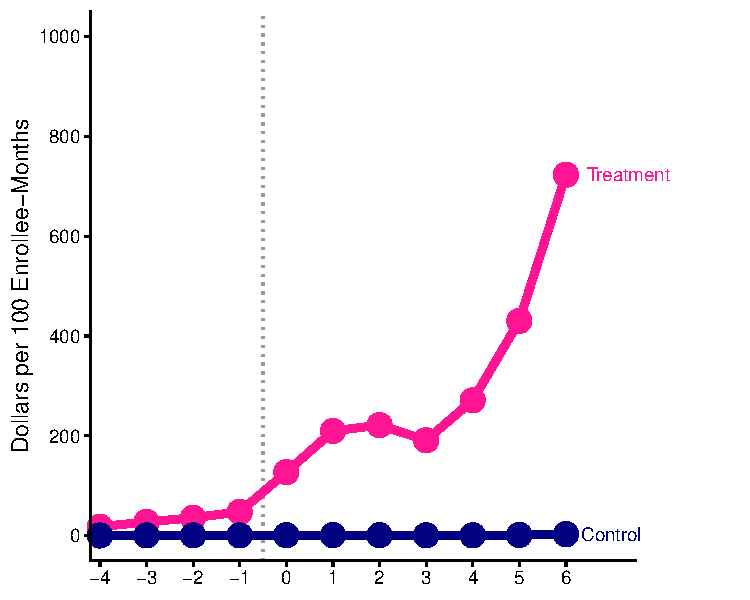
\includegraphics[width=\textwidth]{outputs/figures/emw_weighted/10state/levels_10state_spending_obesity.pdf}
    \label{fig:emw_levels_spending_10state_obesity}
  \end{subfigure}
  \hfill
  \begin{subfigure}[t]{0.48\textwidth}
    \caption{Diabetes GLP-1 Spending\\{\small (10 State Design)}}
    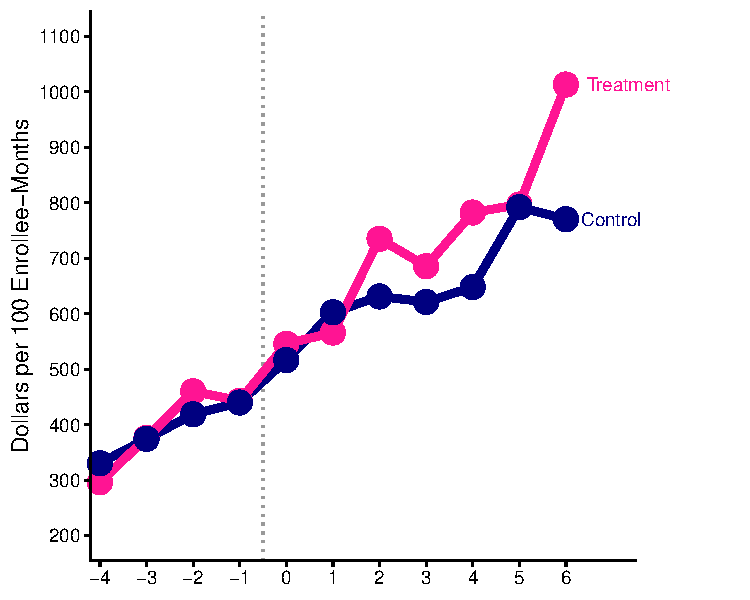
\includegraphics[width=\textwidth]{outputs/figures/emw_weighted/10state/levels_10state_spending_diab_cardiac.pdf}
    \label{fig:emw_levels_spending_10state_diab}
  \end{subfigure}

  \vspace{1em}

  \begin{subfigure}[t]{0.48\textwidth}
    \caption{Obesity GLP-1 Spending\\{\small (7 State Design)}}
    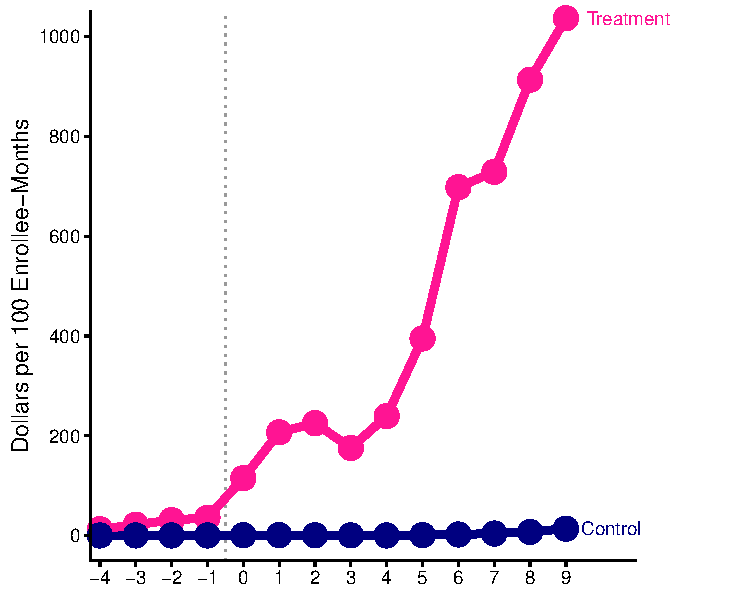
\includegraphics[width=\textwidth]{outputs/figures/emw_weighted/7state/levels_7state_spending_obesity.pdf}
    \label{fig:emw_levels_spending_7state_obesity}
  \end{subfigure}
  \hfill
  \begin{subfigure}[t]{0.48\textwidth}
    \caption{Diabetes GLP-1 Spending\\{\small (7 State Design)}}
    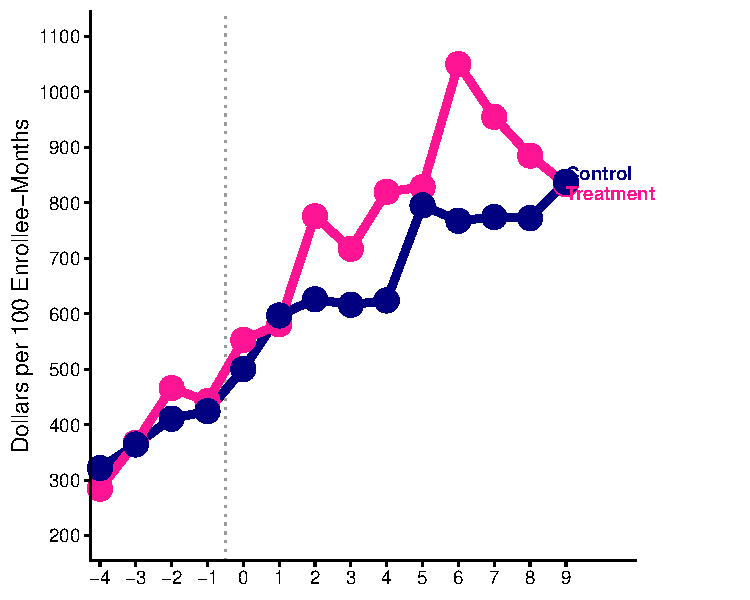
\includegraphics[width=\textwidth]{outputs/figures/emw_weighted/7state/levels_7state_spending_diab_cardiac.pdf}
    \label{fig:emw_levels_spending_7state_diab}
  \end{subfigure}

  \caption{Mean GLP-1 spending levels by event time for treatment and control groups (enrollee-month weighted).}
  \label{fig:emw_levels_spending_combined}
\end{figure}
